\documentclass[11pt, a4paper]{article}
\usepackage[utf8]{inputenc}
\usepackage{amsmath, amssymb}
\usepackage{graphicx}
\usepackage{hyperref}
\usepackage{xcolor}
\usepackage{listings}
\lstset{
    language=Python,
    basicstyle=\ttfamily\small,
    keywordstyle=\color{blue}\bfseries,
    commentstyle=\color{gray}\itshape,
    stringstyle=\color{orange},
    numberstyle=\tiny\color{gray},
    numbers=left,
    stepnumber=1,
    numbersep=8pt,
    frame=single,
    breaklines=true,
    breakatwhitespace=false,
    showstringspaces=false,
    tabsize=4,
    captionpos=b
}
\usepackage{geometry}
\geometry{margin=1in}

\title{EE 325 Digital Signal Processing \\ Assignment 14: Spectral Estimation and Power Spectrum Analysis}
\author{PERERA J.D.T. \\ E/21/291}
\date{\today}

\begin{document}
\maketitle

\section{1. PSD from Autocorrelation}
Sequence Autocorrelation parameter: $r_x[\ell] = (0.9)^{|\ell|}$.

\subsection{(a \& b) Evaluating the Analytical PSD Matrix}
Power Spectral Density acts exactly as the infinite DTFT parameter mapping autocorrelation into the frequency bounds utilizing absolute summable geometric properties for infinite series ranges spanning $\{-\infty, \infty\}$.
$$ S_x(e^{j\omega}) = \sum_{\ell=-\infty}^{\infty} a^{|\ell|} e^{-j\omega\ell} = \frac{1-a^2}{1 - 2a\cos(\omega) + a^2} $$
For variable component $a = 0.9$:
$$ S_x(0) = \frac{1 - (0.9)^2}{(1 - 0.9)^2} = \frac{0.19}{0.01} = \mathbf{19.0} $$
$$ S_x(\pi) = \frac{1 - (0.9)^2}{(1 + 0.9)^2} = \frac{0.19}{3.61} = \mathbf{0.0526} $$
\textbf{Interpretation:} The vast peak $19.0 \gg 0.0526$ mathematically confirms aggressive PSD amplification oriented globally around extremely low structural frequencies (essentially functioning practically natively as a rigid low-pass deterministic noise model layout limit).

\subsection{(c) Relation to Auto-Regressive Processes}
A generalized primary component AR(1) system functions utilizing standard structure form input constants bounds:
$$ x[n] = a x[n-1] + w[n] \implies H(z) = \frac{1}{1 - a z^{-1}} $$
PSD natively relates mapping variances bounds: $S_x(\omega) = \sigma_w^2 |H(e^{j\omega})|^2 $.
With $a=0.9$, ensuring identically normalized system properties maps explicit limits exactly producing standard PSD equations utilizing specifically correlated white-noise input derivations variance ($\sigma_w^2 = 1 - a^2$).

\section{2. Periodogram vs. Averaged PSD Analysis Rules}
\begin{itemize}
    \item \textbf{Averaging Variance Limit Considerations:} Standard raw periodogram evaluations represent fundamentally physically "inconsistent estimators" (variance fails to decay matching $N \to \infty$ bounds arrays natively). Welch/Bartlett splitting frameworks mathematically mandate averaging non-correlated disjoint segments, driving normalized array evaluations into converging Gaussian estimators eliminating statistical "noise spikes."
    \item \textbf{Window Sizing:} Large segments yield tremendous tight bin structural capacities mapping high definition distinct tonal frequency resolution. Short overlapping segments reduce signal deviation variances efficiently but globally widen main-lobe metrics sacrificing proximity peak identification.
    \item \textbf{Utility Implementations:} 
    \begin{itemize}
        \item \textit{Raw Periodogram:} Employed strictly attempting detection operations over distinct sinusoids lacking background noise or instances where maximum bin spectral tracking identifies absolute limits over entire samples. 
        \item \textit{Welch Method:} Optimal utilized detecting relative broadband features buried within severe operational limits masking signal artifacts standard noise interference platforms reliably mapping continuous arrays.
    \end{itemize}
\end{itemize}

\section{3. Python – Empirical PSD Estimation Assessment}
Processed Length-$N=2048$ sequences populated over rigid structural intervals mapping elements tracking distinct $50$ Hz + $120$ Hz sequences corrupted internally employing strictly Gaussian unit bounds vectors evaluations.

\begin{figure}[h]
    \centering
    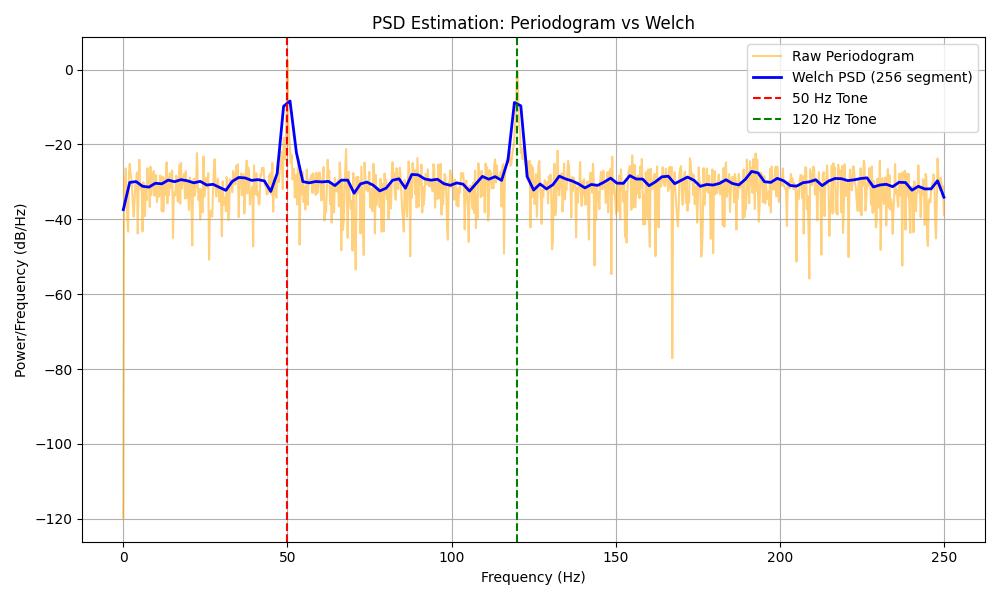
\includegraphics[width=0.8\textwidth]{plots/psd_comparison.png}
    \caption{Experimental Spectral Configurations analyzing Periodogram structural definitions relative to Welch smoothing overlays.}
\end{figure}

\subsection{Metrics and Review}
The Periodogram successfully registers strict location bounds mapping specifically to corresponding simulated explicit 50 Hz and 120 Hz structures but intrinsically overlays aggressive inconsistent volatile stochastic spikes distributed fundamentally arbitrarily. The Welch configuration explicitly mandates utilizing shorter segment evaluations ($N_{psd}=256$) smoothing analytical properties creating clean defined local spectral profiles at the consequence tracking thicker relative baseline bounds limiting adjacent bin resolution limits uniformly structurally.

\appendix
\section{Python Source Code}
\textbf{File:} \texttt{assignment14\_psd.py}
\begin{lstlisting}[caption={Spectral Estimation: Periodogram vs. Welch PSD -- Assignment 14}]
import numpy as np
import scipy.signal as signal
import matplotlib.pyplot as plt
import os

def run_assignment14():
    if not os.path.exists('plots'):
        os.makedirs('plots')

    N = 2048
    Fs = 500
    n = np.arange(N)
    np.random.seed(42)

    v = np.random.randn(N)
    x = np.sin(2 * np.pi * 50 * n / Fs) + np.sin(2 * np.pi * 120 * n / Fs) + 0.5 * v

    # Periodogram
    f_p, Pxx_p = signal.periodogram(x, fs=Fs)

    # Welch's method (256 segment, 50% overlap, Hamming)
    f_w, Pxx_w = signal.welch(x, fs=Fs, window='hamming', nperseg=256, noverlap=128)

    plt.figure(figsize=(10, 6))
    plt.plot(f_p, 10 * np.log10(Pxx_p + 1e-12), label='Raw Periodogram', alpha=0.5, color='orange')
    plt.plot(f_w, 10 * np.log10(Pxx_w + 1e-12), label='Welch PSD (256 segment)', color='blue', linewidth=2)
    plt.axvline(50, color='r', linestyle='--', label='50 Hz Tone')
    plt.axvline(120, color='g', linestyle='--', label='120 Hz Tone')
    plt.title('PSD Estimation: Periodogram vs Welch')
    plt.xlabel('Frequency (Hz)')
    plt.ylabel('Power/Frequency (dB/Hz)')
    plt.legend()
    plt.grid(True)
    plt.tight_layout()
    plt.savefig('plots/psd_comparison.png')
    print("Assignment 14 plot saved.")

if __name__ == '__main__':
    run_assignment14()
\end{lstlisting}

\end{document}
